\section{Vista lógica}

La vista lógica de UbicAR sigue un patrón de arquitectura en capas para garantizar la escalabilidad y el mantenimiento. Se divide principalmente en tres niveles:

\begin{itemize}
    \item \textbf{Capa de Aplicación(Frontend):} Contiene la lógica de la interfaz de usuario, el motor de renderizado de Realidad Aumentada y la gestión de sensores del dispositivo móvil.
    
    \item \textbf{Capa de Servicio(API/Backend):} Actúa como intermediario, procesando las solicitudes de rutas y filtrando la información de profesores y salones antes de enviarla al móvil.

    \item \textbf{Capa de Persistencia:} Encargada de la comunicación con la base de datos SQL Server para recuperar horarios y coordenadas geográficas.
\end{itemize}

\begin{figure}[H]
		\centering
		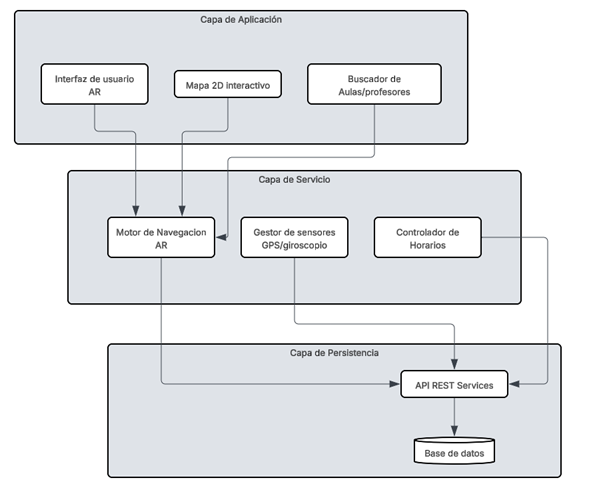
\includegraphics[width=0.95\textwidth]{imagenes/vista-logica.png}
		\caption{Diagrama de Capas de la Vista Lógica}
		\label{fig:vista-logica}
	\end{figure}
